\documentclass[..thesis.tex]{subfiles}

\newtheorem{defin}{Definition}[section]
\newtheorem{kleene-fix}{Theorem}[section]

\begin{document}

\toask{Think subsectioning is needed, also subsectioned the motivational section, guess it would be wise to keep the same style.}
\toask{General style question, I use ``we'' everywhere, comes naturally. Better style available?}
\toans{Yes, you can use `we'' to speak for the scientific community, as in ``we define''. When describing your own contribution, though, you should use ``I''. Many people here use ``the author'', but contemporary English academic writing prefers ``I''.}

\toguide{What is static analysis?}


Under \textit{program analysis} (or just \textit{analysis}) we mean a process of deciding whether some property holds for a program under analysis.
Analysis of a program is \textit{static} if the program being analyzed does not get executed during the analysis, in contrast to \textit{dynamic} analysis,
during what program is executed. Static analysis are often used by compilers, for example for finding uses of variables that are not declared beforehand
in Java or C programs. In addition, modern IDEs constantly run wide selection of static analysis in the background, to enable things such as variable renaming,
for what one would have to know about all the usages of a specific variable in the program, taking into account the relevant scopes. 

\toguide{Why limit ourselves?}


There are good reasons for preferring static analyses over dynamic (or combined) analysis.
To pick a few, it lets us say something about a program that does not compile (and as such, cannot be analyzed dynamically),
it allows to perform our analyses faster compared to dynamic analysis what one cannot perform faster than the time it takes to execute the program
and as static analyses do not depend use any information gathered from a specific run then it is possible to have an analysis that says something
about all the possible runs of a program (and not only, say, for all the possible runs that the analysis has witnessed).
\tosup{About programs that do not compile, a more important category are open programs, such as modules and device drivers, that do not compile alone, but can be analyzed without the rest of the system, so not just considering all runs, but under all possible behaviours of the environment.}
The last reason is, as one can imagine, very helpful in case of data-races. This enables static analysis to output to find that there
 are no errors in the program instead of that it is not able to find any errors -- to verify a program instead of testing it.
 \tosup{Grammar is an issue. You should run a proper grammar check and then try to find someone to check it. One way is to detex -n file.tex > out.txt and feed the file to Grammarly.}


\toguide{How is static analysis done?}


As one might guess, there are a lot of techniques that fit the very wide definition given for static analysis. We will be focusing on one of them --- \textit{abstract interpretation}.
\tosup{Add something like ``unlike most static checkers found in IDEs, abstract interpretation does not simply search for bug patterns; instead, it attempts to compute all possible behaviors of the system in a way that is mathematically reliable.'' I have no idea what mathematical reliability means, but it sounded believable.}

\toguide{Okay, what is abstract interpretation?}


To give an intuition on what is abstract interpretation, consider following program:

\begin{lstlisting}[language=C,style=def]
int main(void) {
  int x, y, z;
  x = 0;
  y = -81;
  z = -37
  if (y * z > 0){
    x = 1;
  }
  return x;
}
\end{lstlisting}

One can easily deduce that the program will always exit with error code $1$, without having to calculate the exact value of  $y*z$.
Instead, we can interpret all the values variables have as negative ($-$), $0$ or positive ($+$) and evaluate $y * z$ as $-*- = +$.

This is considerable easier task.

With this simplification, we do lose precision. Lets consider another example:

\begin{lstlisting}[language=C,style=def]
int main(void) {
  int x, y, z;
  x = 0;
  y = -81;
  z = -37;

  if (y * z > 0){
    x = 1;
  }

  if (y * z - y > 0){
    x = 2;
  }
  return x;
}
\end{lstlisting}.


Here, using the interpretation what we successfully applied in previous example, we would not be able to decide the return value of the program. 
When evaluating $y * z - y $, we can rule out any of the possible values. To be able to evaluate product in a similar way previously described,
we could assigns variables set of \textit{possible} values instead. In this case, we would evaluate $y * z - y $ as $\left\lbrace - \right\rbrace * \left\lbrace
- \right\rbrace - \left\lbrace - \right\rbrace = \left\lbrace -,0,+ \right\rbrace$. Although we cannot decide what the program will return,
we can decide based on the analysis, that the first $if$ block can safely be ignored -- an optimization a compiler could perform.
\tosup{You will need to check the typography at some point, $if$ is definitely not what you want here.}

\subsection{Concrete semantics}

To build a mathematically sturdy foundation for abstract interpretation we first need to give a more formal definition for executing a program.
This is known as its \emph{concrete semantics}.
 For that, lets give a formal definition of a program.
\tosup{I'd rather say that we work on a common intermediate representation (IR), the control flow graph, or programs are represented as flow graphs, rather than this being the definition of a program.}

\begin{defin}
Procedure $p$ is a \textit{control flow graph} $\left( N_p,E_p,s_p,r_p \right)$, where $N_p$ is a finite set of nodes, $s_p \in N_p$
 is the \textit{entry} node with in-degree $0$ and  $r_p \in N_p$ is the \textit{return} node with out-degree $0$. Set of labels $L$ consists of
\begin{itemize}
\item statements $s \in Stmt$, other than procedure calls.
\item procedure calls $p()$, where $p \in Exp$ is an expression, 
\item positive and negative guards ( $Pos\left( e \right) in Guards$ and  $Neg \left( e \right) \in Guards$, $e \in Exp$),
\item and thread spawning function $spawn\left( e \right), e \in Exp$.  
\end{itemize}
The edge set  $E_p \subseteq N_p \times L \times N_p$. In addition, we require that out-degree of node $n \in N_p$ is no bigger than $2$ 
and if $e_1$ and $e_2$ are outgoing edges of $n$ and $e_1 \neq e_2$, then one of $e_1$ and $e_2$ is a positive guard and other a negative guard. 
\end{defin}
\tosup{These restrictions on the outgoing edges is probably not needed for correctness of our framework.}

It is worth mentioning that although we have constrained ourselves with procedure calls without any arguments and only one return node,
 those issues can be easily solved with use of global variables. 

In addition, we assume that for every $n \in N_p$, there exists a path from $s_p$ to $n$ and from $n$ to $r_p$. \toadd{do I need this?} 

\begin{defin}
Program $P = \left( Proc, main \right)$, where $Proc$ is a finite set of procedures such that for every $p,q \in Proc, p \neq q \implies N_p \cap N_q = \emptyset$ 
and $main \in Proc$ is one of the procedures designated as the main function.
 Let $N$ be set of all nodes in the program, that is $N = \bigcup_{p \in Proc}N_p$ and $E$ be a set of all edges in the program, that is $E = \bigcup_{p \in Proc}E_p$. 
\end{defin}


\begin{figure}[H]
  \centering
  \begin{tikzpicture}[node distance=2cm]

    \node (start) [end] {$s_{main}$};
    \node (decl) [node, below of=start] {};

    \node (assign_x) [node,below of=decl] {};
    \node (assign_y) [node,below of=assign_x] {};
    \node (assign_z) [decision,below of=assign_y] {};

    \node (x_assign_1) [node, below right of = assign_z] {};

    \node (if_y_times_z_minus_y) [decision,below left of = x_assign_1] {};
    \node (x_assign_2) [node, below right of = if_y_times_z_minus_y] {};

    \node (after_second_if) [node, below left of = x_assign_2] {};

    \node (end) [end, below of  =  after_second_if] {$r_{main}$};

    \draw [arrow] (start) -- node [anchor=west] {\cfgcode{int x, y, z}} (decl);

    \draw [arrow] (decl) -- node [anchor=west] {\cfgcode{x = 0}} (assign_x);
    \draw [arrow] (assign_x) -- node [anchor=west] {\cfgcode{y = -81}} (assign_y); 
    \draw [arrow] (assign_y) -- node [ anchor=west] {\cfgcode{z = -37}} (assign_z);
      
    \draw [arrow] (assign_z) --
      node [ anchor=west] {\cfgcode{Pos(y * z > 0)}} (x_assign_1);
    \draw [arrow] (x_assign_1) -- node [ anchor=west] {\cfgcode{x = 1}} (if_y_times_z_minus_y);

    \draw [arrow] (assign_z) --
      node [ anchor=east] {\cfgcode{Neg(y * z > 0)}} (if_y_times_z_minus_y);
   
        
    \draw [arrow] (if_y_times_z_minus_y) --
      node [ anchor=west] {\cfgcode{Pos(y * z  - y > 0)} } (x_assign_2);
    \draw [arrow] (x_assign_2) -- node [ anchor=west] {\cfgcode{x = 2}} (after_second_if);

    \draw [arrow] (if_y_times_z_minus_y) --
      node [ anchor=east] {\cfgcode{Neg(y * z - y > 0)}} (after_second_if);
      
    \draw [arrow] (after_second_if) -- node [ anchor=west] {\cfgcode{return x}} (end);

  \end{tikzpicture}
  \caption{CFG corresponding to the last code snippet}
\end{figure}

\toask{Should listings be given names? Seems bit too heavyweight to wrap them in figures, but would make citing so much easier}
\toans{I would probably prefer code listings to be separate floating with own caption, but this is not really a high-priority issue.}

As it is not feasible to offer a formalization of all the statements and expressions available in any of common higher-level programming languages
as a part of this thesis, we have elected to leave the sets $Stmt$ and $Exp$ formally undefined, instead relying on the reader's previous experience
with statements and expressions in any of the C family languages.   For the interested, a formalization of a subset of C is done by Vojdani \toadd{Cite to doctoral thesis}.

\toask {very clumsy, but would like to bring this up and not just leave the sets undefined}

\toguide{So, what can we do with this program?}

\toask{Subsectioning?}

Now that we have defined how program looks, we will continue with how such a program is evaluated -- the \textit{semantics} of the program.

From here on we will use following notation to ``update'' a function:

\begin{equation*}
f \left[ x : a \right] \left( y \right) = 
  \begin{cases}
  a & y = x \\
  f \lp  y \rp & otherwise \\ 
  \end{cases}
\end{equation*}.

Lets first consider single threaded programs. Let $S$ be set of states of the program, that is $s : Var \to Val$, where $Var$ is set of
variables in the program and $Val$ is set of possible values. Again, we will not formally define sets $Val$ and $Var$ here.
For every statement $stmt \in Stmt$, let $ \lllb s \rrrb_{Stmt} : S \to S$ be a function that updates the state of the program. 
\tosup{Whoa, $s$ is used for everything!}

For example

\begin{equation*}
 \lllb x = 3 \rrrb_{Stmt} (s) = s \left[ x : 3 \right] \text{.}
\end{equation*}

Similarly, for every expression $e \in Exp$, let $\lllb e \rrrb_{Exp} : S \to Val$ that evaluates expression in context of the state. 

For example, let $s$ be a state after assigning $3$ to $x$, that is

\begin{equation*}
s = \lllb x = 3 \rrrb_{Stmt} (s_0) \text{,}
\end{equation*},
where $s_0$ is an arbitrary state. 

Then 
\begin{equation*}
\lllb x + 8 \rrrb_{Exp} \left( s \right) = 11 \text{.}    
\end{equation*}

With this in mind, we can define a relation for intra-procedural evaluation of our programs as follows:

\begin{defin}
Intra-procedural evaluation relation of procedure $p$, $\intraproc_p \subseteq  \lp N_p  \times S \rp  \times \lp N_p \times S \rp$
is a relation for what following rules hold:
\tosup{I'm not currently concerned with grammar, but globally ``for what'' $\to$ ``for which''!}

\addtolength{\jot}{2em}
\begin{gather*}
  \inference[Stmt]{ \lp u, stmt, v \rp \in E_{p}  \separ  \lllb stmt \rrrb_{Stmt} \lp s \rp = s'}{\lp u, s \rp \intraproc \lp v, s' \rp} \\
  \inference[Pos]{ \lp u, Pos \lp e \rp , v \rp \in E_{p} \separ \lllb e \rrrb_{Exp} \lp s \rp = true }{\lp u, s \rp \intraproc \lp v, s \rp} \\  
  \inference[Neg]{ \lp u, Neg \lp e \rp , v \rp \in E_{p} \separ \lllb e \rrrb_{Exp} \lp s \rp \neq true }{\lp u, s \rp \intraproc \lp v, s \rp} 
\end{gather*}
\addtolength{\jot}{-2em}

\end{defin}

\tosup{So I would probably get rid of this index $p$ on the $\intraproc_p$, but if you keep it, note that it is currently missing in the rules. Why do you need a relation per procedure? It also clutters the next rules.}

This relation gives a formal definition for one atomic step during evaluation of a procedure, when evaluating a procedure step with the relation $\intraproc$,
the rule applied depends on the type of the edge under evaluation. 

\toguide{ What about procedure calls?}

To support inter-procedural evaluation of our program, we need to keep track of the caller of process. For that we will use, as is usually done, a \textit{call stack}.
Call stack is a tuple of CFG nodes, first node is current CFG node (the one being evaluated) and rest of nodes are call sites, points from where program evaluation
 should continue after reaching the return node. Let $Stack$ be set of all call stacks of program $P$. 

We will define inter-procedural evaluation relation for single-threaded program $P$ as follows:

\begin{defin}

Inter-procedural evaluation relation of single-threaded program $P$, 
$\interproc \subseteq \lp Stack \times S \rp \times \lp Stack \times S \rp$ 
is a relation for what following rules hold:

\addtolength{\jot}{2em}
\begin{gather*}
  \inference[Stmt]{\lp u, stmt, v \rp \in E  \separ \exists p \in P  \lp u, s \rp \intraproc_p \lp v, s' \rp }{ \lp u :: xs, s \rp \interproc \lp v :: xs, s` \rp} \\
  \inference[Pos]{ \lp u, Pos \lp e \rp, v \rp \in E \separ   \lllb e \rrrb_{Exp} \lp s \rp = true  }{\lp u :: xs , s \rp \interproc \lp v :: xs, s \rp} \\ 
  \inference[Neg]{ \lp u, Neg \lp e \rp, v \rp  \in E \separ   \lllb e \rrrb_{Exp} \lp s \rp \neq true  }{\lp u :: xs , s \rp \interproc \lp v :: xs, s \rp} \\
  \inference[Call]{ \lp u, p\lp\rp , v \rp  \in E \separ  \lllb p \rrrb_{Exp} \lp s \rp = proc \separ proc \in Proc }{\lp u :: xs , s \rp \interproc \lp s_{proc} :: v :: xs, enter_{proc} s \rp} \\
  \inference[Return] { proc \in Proc} { \lp r_{proc}::xs , s \rp \interproc \lp xs, return_{proc} s \rp}
\end{gather*}
\addtolength{\jot}{-2em}

where $enter_{proc}$ and $return_{proc}$ are state transformers that initialize and destroy local variables.
\end{defin}
\tosup{Make sure you are consistent with $p$ versus $proc$; it seems entirely random above.}
\tosup{Why are there separate Pos and Neg rules?? This defeats the purpose of having a separate intra-proc semantics. Can't you just make a transition whenever the intra one can do it?}

\toguide{What about threads?}

To support multithreaded programs, we will first expand our inter-procedural evaluation relation to support the thread spawning function $spawn$.
\tosup{Might want to anticipate future developments: ``we will first lift our inter-procedural evaluation relation to a semantics of executing individual threads, which supports the spawning of other threads. We will later use this to define a semantics that takes thread interleavings into account.''}

\begin{defin}

  Intra-thread evaluation relation of $P$,

  \begin{equation*}
    \intrathread \subseteq  \lp Stack \times S \rp \times \lp Stack \times S \times Proc^\ast \rp
  \end{equation*}

  is a relation for what following rules hold:

  \addtolength{\jot}{2em}
  \begin{gather*}
    \inference[Spawn]{\lp u, spawn(p), v \rp \in E  \separ  \lllb p \rrrb_{Exp} = proc \separ proc \in Proc  }{ \lp u :: xs, s \rp \intrathread \lp v :: xs, s, (proc) \rp} \\
    \inference[Pos,Neg,Call,Return] {\lp u, stmt, v \rp \in E \separ \lp xs , s \rp \interproc \lp ys, s' \rp }{ \lp xs , s \rp \intrathread \lp ys, s', \lp \rp \rp}
  \end{gather*}
  \addtolength{\jot}{-2em}

\end{defin}

\toask{ Okay, but the process list is not used anywhere?}

The added information about spawned threads will be used by the following relation.

\begin{defin}

  The inter-thread evaluation relation of $P$, 
 
  \begin{equation*}
    \interthread \subseteq \lp Stack^\ast \times S \rp \times \lp Stack^\ast \times S \rp
  \end{equation*}

  is a relation for what following rule holds:   

  \begin{equation*}
    \inference{ 0 \leq i \leq n  \separ \lp t_i , s \rp \intrathread \lp t'_i, s', \lp p_1^\star, \ldots, p_k^{\star} \rp \rp}{ \lp \lp t_0, \ldots, t_n \rp, s \rp \interthread  \lp \lp t_0, \ldots, t_n, \lp s_{p_1^{\star}} \rp, \ldots, \lp s_{p_k^{\star}} \rp  \rp , s' \rp} \text{.}
  \end{equation*}

  \tosup{I injected $t_i$ above, but you should inject it below as well. Question: why are the spawned threads $p$-s with a star. That would seem like they are a list or something? I'm also wondering if maybe square brackets would be better for lists to make clearer that you have singleton call stacks.}
\end{defin}

In the $\lp \interthread \rp$ relation, the list of stacks corresponds to call stacks of all the threads currently running.
It is worth noting that relation $\lp \interthread \rp$ is non-deterministic if there is more than one thread in the program -- a property that multithreaded programs have.

The $\lp \interthread \rp$ lets us define a set of all possible states of a program $P$, with starting state $s_0$ :

\begin{equation*}
\allstates = \left\lbrace  z | \lp \lp s_{main} \rp, s_0 \rp \interthread^{\ast} z \right\rbrace \text{.}
\end{equation*}


\toask{So, what is the point of this?}

Equipped with set \allstates we would have information about the program at any possible execution point. At the same time,
 it is clear that computing the set \allstates is not feasible in most cases --- the set might not be finite and even if it is,
 the all possible states of even a simple program might be quite big.

\subsection{Abstract domains}

As in the example we gave at the start of this section, we can however simplify the program by \textit{abstracting} away parts
of the state that are not interesting for us for finding out if a certain property holds for the program under analysis. 
However, it is not easy to get the level of abstraction right, as abstracting away too much does not let us tell much about non-trivial properties
of the program and abstracting away too little leaves us with task that is too big to feasibly compute.

\toask{So, how are we abstracting?}

To have our abstraction on a sound footing, we need a formalization of the idea.
 The mathematical theory of \textit{complete lattices} offers a suitable framework.
 We will now give a short introduction to the lattice theory.

\toask{Okay, lattice theory?}

First of all, a quick reminder from set theory.

\begin{defin}[Partial Order]
A set $D$ with relation $\sqsubseteq \subseteq D \times D$ is called a \textbf{partially ordered set} if $\sqsubseteq$ 
is a \textbf{partial order}, that is reflexive, antisymmetric and transitive.
\end{defin}
\tosup{Try to avoid notation like $\sqsubseteq \subseteq D \times D$. I think you can just assume people know what a relation is, and if they don't, this is even harder for them to parse.}

\begin{defin}[Upper bound]
Let $\lp D, \sqsubseteq \rp$ be a partially ordered set. An \textbf{upper bound} of set $X \subseteq D$,  is an element $x \in D$, such that for every element in $y \in X$, $y \sqsubseteq x$. Element $x$ is the \textbf{least upper bound} of set $X$, denoted as $\bigsqcup X$ if for every other upper bound $z$ of $X$, $x \sqsubseteq z$.  
\end{defin}

\begin{defin}[Lower bound]
Let $\lp D, \sqsubseteq \rp$ be a partially ordered set. An \textbf{lower bound} of set $X \subseteq D$  is an element $x \in D$, such that for every element in $y \in X$, $x \sqsubseteq y$. Element $x$ is the \textbf{greatest lower bound} of set $X$, denoted as $\bigsqcap X$ if for every other lower bound $z$ of $X$, $z \sqsubseteq x$.    
\end{defin}

Equipped with these three definitions, we can now define \textit{complete lattice}:

\begin{defin}[Complete lattice]
A tuple $\lp D, \sqsubseteq \rp$ is a complete lattice if $D$ is a partially ordered set with relation $\sqsubseteq$ and for every set $X \subseteq D$, there exists $\bigsqcup X$ and $\bigsqcap X$.
\end{defin}


We will use notation $x \sqcup \lp  \sqcap \rp y$ to denote $\bigsqcup \lp \bigsqcap \rp \lb x, y \rb$ and $\bot$ to denote the least element in $D$, that is $\bot = \bigsqcap D$ and $\top$ to denote the greatest element in D, $\top = \bigsqcup D$.
\tosup{Do not use parenthetical conventions in mathematical definitions. This $\bigsqcup \lp \bigsqcap \rp \lb x, y \rb$ looks like some weird expression. Spell it out or say it's analogous.}

\toask{So many definitions, what is this (complete) lattice thing?}

Lets now have a look at couple of examples. 

First of all, let $D$ be $\lb true, false \rb$ and let $\sqsubseteq = \lb \lp false, true \rp \rb$. Then $true = \top = \bigsqcup D$ and $false = \bot = \bigsqcap D$. An usual way to describe lattices is the use of Hasse diagrams, graphs that have as nodes the elements of $D$ and there is an edge between $u, v \in D$ if $u \sqsubseteq v$. The edges that are implied by reflexivity or transitivity are usually omitted.
\tosup{Again, this $\sqsubseteq = \lb \lp false, true \rp \rb$ looks weird just say ``with the ordering $\mathit{false} \sqsubseteq \mathit{true}$.}

\begin{figure}[H]
  \begin{center}
    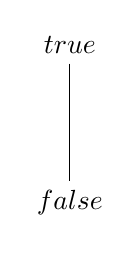
\begin{tikzpicture}
      \node (true) at (0,1) {$true$};
      \node (false) at (0,-1) {$false$};
      \draw (true) -- (false);
    \end{tikzpicture}
  \end{center}
  \caption{$\lp \lb false, true \rb, \lb \lp false, true \rp \rb \rp$ as an Hasse diagram.}
\end{figure}
 
Secondly, in the example we used to gain intuition about abstract interpretation, we gave each variable a set of its possible values at that program state. Under the values we differentiated between negative integers, zero and positive integers. The corresponding lattice would be the following.


\begin{figure}[H]
  \begin{center}
    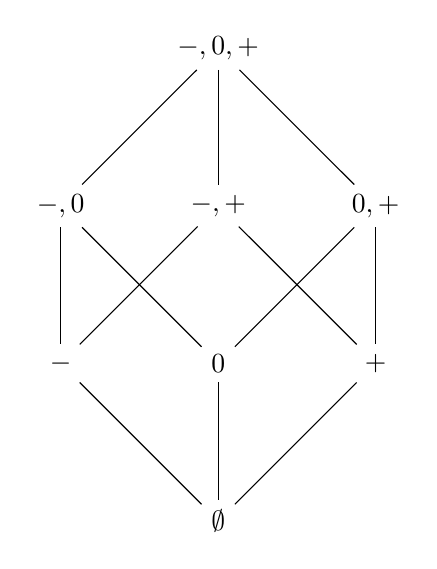
\begin{tikzpicture}
      \node (D) at (0,2) {$\lb -,0,  + \rb$};

      \node (minuszero) at (-2,0) {$\lb -, 0 \rb$};
      \node (minusplus) at (0,0) {$\lb -,+ \rb$};
      \node (zeroplus) at (2,0) {$\lb 0,+ \rb$};

      \node (minus) at (-2,-2) {$\lb - \rb$};
      \node (zero) at (0,-2) {$\lb 0 \rb$};
      \node (plus) at (2,-2) {$\lb + \rb$};

      \node (empty) at (0,-4) {$\emptyset$};

      \draw (D) -- (minuszero);
      \draw (D) -- (minusplus);
      \draw (D) -- (zeroplus);

      \draw (minuszero) -- (minus);
      \draw (minuszero) -- (zero);

      \draw (minusplus) -- (minus);
      \draw (minusplus) -- (plus);

      \draw (zeroplus) -- (zero);
      \draw (zeroplus) -- (plus);

      \draw (minus) -- (empty);
      \draw (zero) -- (empty);
      \draw (plus) -- (empty);
    \end{tikzpicture}
  \end{center}
  \caption{$2^{\lb -, 0, + \rb}$, ordered by inclusion}
\end{figure}

It is worth noting that for every set $S$, its powerset $2^S$ is a complete lattice when ordered by inclusion with union of two sets being the least upper bound and intersection being the greatest lower bound.

As a last example, lets look at \textit{flat lattice} -- a lattice defined on a set $S \cup \lb \bot, \top \rb$, with following ordering $\sqsubseteq = \lb \lp  u,v \rp  | u = \bot \land v \in S \lor  u \in S \land  v = \top \rb$. For a concrete example, let $S$ be $\mathbb{Z}$.

\begin{figure}[H]
  \begin{center}
    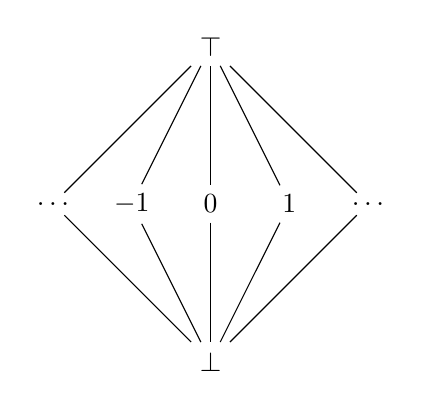
\begin{tikzpicture}
      \node (top) at (0,1) {$\top$};

      \node (neg) at (-2,-1) {$\ldots$}; 
      \node (minus_one) at (-1,-1) { $-1$ };
      \node (zero) at (0,-1) { $0$};
      \node (one) at (1,-1) { $1$ };
      \node (pos) at (2,-1) {$\ldots$}; 

      \node (bot) at (0,-3) {$\bot$};

      \draw (top) -- (neg);
      \draw (top) -- (minus_one);
      \draw (top) -- (zero);
      \draw (top) -- (one);
      \draw (top) -- (pos);

      \draw (neg) -- (bot);
      \draw (minus_one) -- (bot);
      \draw (zero) -- (bot);
      \draw (one) -- (bot);
      \draw (pos) -- (bot);

    \end{tikzpicture}
  \end{center}
  \caption{the flat lattice of $\mathbb{Z}$ }
\end{figure}

The flat lattice is one way to create a complete lattice from any kind of set.

\toask{Okay, but what it has anything to do with abstract interpretation?}

Lattices will serve as \textit{abstract domains} for abstract interpretation. Intuitively, the elements of abstract domain will fulfill the same role as the states in concrete interpretation, offering context for interpreting the program. For abstract domain (that is, a complete lattice) $D,\sqsubseteq$, we will choose $D$ to be a (finite) set of elements that each describe some set of states of our concrete implementation. To analyze the program we would like to find the most precise element of $D$ -- that is, that describes the least amount of states in our concrete implementation, while describing that specific state for every state in our program. So, an \textit{analysis} of program $P$ is a function $\analyze : N \to D$.
\tosup{Why does $D$ need to be finite?}
\tosup{I don't understand what is meant with ``while describing that specific state for every state in our program''.}

For our running example, as we care only about the signs of variable, a suitable $D$ would be a set of functions from set of all variables in program $P$ to power set of $\lb -, 0, + \rb$, that is $d \in D, d : Var_P \to 2^{\lb -, 0, + \rb}$. 
$D$ is ordered point-wise, that is $d_1 \sqsubseteq d_2 \iff \forall v \in Var_p, d_1 v \subseteq d_2 v$. 
\tosup{You need a global sweep to \\mathitify variables, but this $Var$ is particularly bad.}

\toguide{Is that even a lattice?}

It is worth noting that $D$ is also a lattice as for every subset $X$,
\begin{equation*}
  \bigcup X = \lb \lp v, b \rp | \forall v \in Var, b = \bigcup \lb d \lp v \rp | d \in X \rb \rb
\end{equation*}
and $\bigcap X$ is defined dually.

\toask{Is dually even a word and if so, does it get the point across?}

\toguide{So, why bother with the lattice, what does it give us?}

One might still be wondering, why do we want to use lattices here, instead of simple sets. Consider following program.

\begin{figure}[H]
  \begin{center}
    \begin{tikzpicture}[node distance=2cm]

      \node (start) [end] {$s_{main}$};
      \node (decl) [decision, below of=start] {$1$};

      \node (rand_pos) [node,below right of = decl] {$3$};
      \node (rand_neg) [node, below left of = decl] {$2$};

      \node (after_if) [node, below left of = rand_pos] {$4$};

      \node (end) [end, below of = after_if] {$r_{main}$};

      \draw [arrow] (start) -- node [anchor=west] {\cfgcode{int x }} (decl);

      \draw [arrow] (decl) --
        node [ anchor=west] {\cfgcode{Pos(rand() \% 2 == 0)}} (rand_pos);
      \draw [arrow] (rand_pos) -- node [ anchor=west] {\cfgcode{x = 1}} (after_if);

      \draw [arrow] (decl) --
        node [ anchor=east] {\cfgcode{Neg(rand() \% 2 == 0)}} (rand_neg);
      \draw [arrow] (rand_neg) -- node [ anchor=east] {\cfgcode{x = 0}} (after_if);   
      
      \draw [arrow] (after_if) -- node [ anchor=west] {\cfgcode{return x}} (end);

    \end{tikzpicture}
  \end{center}
  \caption{An example program}
\end{figure}


When taking the $Pos$ edge in the example program then the most precise element of the domain that would describe the state at node $4$ would be $d_1 = \lb \lp x, \lb + \rb \rp \rb$. When taking the $Neg$ edge, the most precise element for describing state at node $4$ would be $ d_2 = \lb \lp x, \lb 0 \rb \rp \rb$. However, based on static analysis, it is not possible to say which edge will be picked as it depends on a random number generated during runtime. In this case, we would like to describe the state at node $4$ with an element from domain that describes the state most precisely, taking into account that either of the conditional branches could be taken. Based on how we have constructed this domain, the suitable element would be $d_1 \bigsqcup d_2 = \lb \lp (x, \lb 0, + \rb \rp \rb$.

To be able to use the least upper bound when joining information from different possible incoming edges to state, the domain should be ordered in a way that if $d_1 \sqsubseteq d_2$ then if a property $P$ that we are interested in holds for $d_1$, it should always hold for $d_2$ as well. More concisely, $d_1 \sqsubseteq d_2 \implies\lp  P \lp d_1 \rp \implies P \lp d_2 \rp \rp$.

In our example, the properties we were considering were whether a specific variables value \textit{may} be positive, negative or zero. If the value of a variable may be $0$, then it also may be $0$ or positive so we would want $\lb 0 \rb \sqsubseteq \lb 0, + \rb$. However, if we would wonder about whether a specific variable value would \textit{not} be positive, negative or zero then if we know that if the value is not 0 or positive then it also is not zero, meaning that we would want to have a lattice $\lp 2^{-,0,+}, \sqsubseteq_{must} \rp$ such that $\lb 0 , + \rb \sqsubseteq_{must} \lb 0 \rb$. We could define $\sqsubseteq_{must}$ to be

\begin{equation*}
d_1 \sqsubseteq_{must} d_2 \iff d_2 \sqsubseteq d_1 \text{.} 
\end{equation*} 

\toguide{Okay, I get the idea with the bounds, but how does this help us?}


More formally, let $P$ be a program, $\allstates$ be set of all the possible states of the program and let $L = \lp D, \sqsubseteq \rp$ be a lattice. We say that $\descriptor \subseteq \allstates \times D$ is a \textit{descriptor relation} if there is no $s \in \allstates$ such that $s \descriptor \bot_L$, for every state $s \in \allstates$, $s \descriptor \top_L$ and for all $d_1,d_2 \in D, s \in \allstates$,

\begin{equation*}
s \descriptor d_1 \land d_1 \sqsubseteq d_2 \implies s \descriptor d_2 \text{.}
\end{equation*}

In concrete interpretation, to evaluate a program statement $\lp v, s, u \rp$ we used function $\lllb s \rrrb_{Stmt} : S \to S$. To evaluate the same program statement in abstract interpretation over domain $D$, we need to define functions $\lllb s \rrrb_{Stmt}^{\absint} : D \to D$, that we can use to evaluate the program in context of domain element $d$. For example, in case of our running example, we could define $\lllb x =  x + 2 \rrrb_{Stmt}^{\absint}$ as

\begin{equation*}
\lllb x = x + 1 \rrrb_{Stmt}^{\absint} \left( d \right) =
\begin{cases}
d \lbk x : \lb + \rb \rbk & d \lp x \rp  \in \lb  \lb 0  \rb, \lb + \rb, \lb 0, + \rb \rb  \\
d \lbk x : \lb -, 0 \rb \rbk & d \lp x \rp =  \lb - \rb \\
d \lbk x : \lb -, 0, + \rb \rbk & d \lp x \rp \in \lb \lb -,0 \rb, \lb -, + \rb, \lb -, 0, + \rb \rb \\
\end{cases}
\text{.}      
\end{equation*}

We demand that the functions $\lllb s \rrrb_{Stmt}^{\absint}$ are consistent to functions $\lllb s \rrrb_{Stmt}$, that is, for each $s \in S, d \in D$ if $s \descriptor d$ then $ \lllb s \rrrb_{Stmt} \descriptor \lllb d \rrrb_{Stmt}^{\absint}$.

\begin{figure}[H]
  \begin{centering}
    \begin{tikzpicture}
      \node (start) at (0,5) {$s = \lb \lp x, 0 \rp \rb$};
      \node (start_a) at (5,5) {$d = \lb \lp x , \lb 0 \rb \rp \rb$};
      \node (end) at (0,0) {$s' = \lb \lp x, 1 \rp \rb$};
      \node (end_a) at (5,0) {$d' = \lb \lp x , \lb + \rb \rp \rb$};
      
      \draw [arrow] (start) -- node[anchor = east] {$s'=\lllb x = x +1  \rrrb_{Stmt} \lp s \rp$}  (end);
      \draw [arrow] (start_a) -- node[anchor = west] {$d'=\lllb x = x + 1 \rrrb_{Stmt}^{\absint} \lp d \rp$} (end_a);
      
      \draw [dashed] (start) -- node[anchor = south] {$s \descriptor d$} (start_a);
      \draw [dashed] (end) -- node[anchor = south] {$s' \descriptor d'$} (end_a);
    \end{tikzpicture}
  \end{centering}
  \caption{The connections between $\allstates$, $D$, $\lllb x = x +1  \rrrb_{Stmt}$ and $\lllb x = x + 1 \rrrb_{Stmt}^{\absint}$.}
\end{figure}

Also, we will want all the functions $\lllb s \rrrb_{Stmt}^{\absint}$ to be \textit{monotonic}.

\begin{defin}
Let $\lp X, \leq_X \rp$ and $Y, \leq_Y$ be partially ordered sets. Then $f : X -> Y$ is \textit{monotonic} if for every $x_1, x_2$, $x_1 \leq_X x_2 \implies f \lp x_1 \rp \leq_y f \lp x_2 \rp$.   
\end{defin}

This requirement is quite natural -- the monotonicy of the evaluation functions means that if we abstractly evaluate a program statement in context of domain element then the resulting state has to be at least as precise as if we would have evaluated the same statement in context of less precise domain element.  


\toask{Quite jump?}
\subsection{Abstract interpretation}
%või Data Flow Analysis või Intra-procedural analysis, kui tuleb pärast protseduurid ja lõimed.

For now, lets limit ourselves to intraprocedural analyses in following.
 
As mentioned before, we want to define analyze $\analyze : N \to D$ such that for every node $n$ in program $P$, every state $s \in \allstates$ that can happen when the execution has reached node $n$, $s \descriptor f \lp n \rp$.
  
Let $n$ be a node in program $P$. Let $w$ be a finite walk in program $P$, starting from state $s_P$ and ending in $n$, that is $w = \lp s_P, stmt_0, s_1, stmt_1, \ldots, s_i, stmt_i, n \rp$. Lets note if $d_s$ is the abstract starting state, that is $s_P \descriptor d_s$  that we can evaluate the edges on this path in the following way:

\begin{equation*}
d_w = \lllb stmt_i \rrrb_{Stmt}^{\absint} \circ \lllb stmt_{i-1} \rrrb_{Stmt}^{\absint} \circ \ldots \circ  \lllb stmt_0 \rrrb_{Stmt}^{\absint} \lp d_s \rp  
\end{equation*}
  
If we define $W_n$ to be the set of all the finite paths from $s_P$ to $n$ in program P, then could now define $f$ as

\begin{equation*}
\analyze \lp n \rp = \bigsqcup \lb d_w \| p \in W_n \rb \text{.} 
\end{equation*}  

\toask{Even bother with introducing MOP? Could try to explain the constraint system through it?}

This approach, knows as \textit{meet over all  paths (MOP)}, has downsides, the most obvious is the possible computational complexity as the number of paths can grow exponentially with the size of the program and, even worse, the number of walks do not have to be finite. Additionally, it is not clear how to handle infinite walks. 

We will be using another approach for defining $\analyze$.

\toask{I would like to convince reader, that the constraint system is natural, but it somehow very difficult. Leave it out or try to approach from another angle?}

Lets consider a specific edge in our program, $\lp v, s, u \rp$. Now, let $d = \analyze \lp v \rp$. Then, presuming that $d$ is precise, $\analyze \lp u \rp $ should not be more precise than $\lllb s \rrrb_{Stmt} \lp d \rp$ as ...

\toadd{Fix this}
  
From this, we get a following constraint system

\begin{equation}
\label{constraints}
\analyze \lp  u \rp \sqsupseteq \lllb s \rrrb_{Stmt} \lp \analyze \lp v \rp \rp ~~ \forall \lp e = \lp u, s, v \rp \rp \in E_P \text{.}
\end{equation}

Additionally, the abstract starting state should also be an lower bound to $\analyze \lp s_P \rp$, so $\analyze \lp s_p \rp \sqsupseteq d_S$. 

We can now define $\analyze$ to be a function that is the least solution to the given constraint system.

\toguide{Hmm, constraint system, need to digest this. An example?}

As an example, lets look at example program $B$: 

\begin{figure}[H]
  \centering
  \begin{tikzpicture}[node distance=2cm]
    \node (start) [end] {$s_{main}$};
    \node (decl) [decision, below of=start] {$1$};

    \node (rand_pos) [node, right  = 4 cm of  decl] {$3$};
    \node (rand_neg) [node, below of = decl] {$2$};

    \node (after_if) [node, below of = rand_neg] {$4$};

    \node (end) [end, below of = after_if] {$r_{main}$};

    \draw [arrow] (start) -- node [anchor=east] {\cfgcode{int x = 0 }} (decl);

    \draw [arrow] (decl) edge [bend left]
      node [ anchor=south] {\cfgcode{Pos(rand() \% 2 == 0)}} (rand_pos);
    \draw [arrow, bend right] (rand_pos) edge [bend left] node [ anchor=north] {\cfgcode{x = x + 1}} (decl);

    \draw [arrow] (decl) --
      node [ anchor=east] {\cfgcode{Neg(rand() \% 2 == 0)}} (rand_neg);
    \draw [arrow] (rand_neg) -- node [ anchor=east] {\cfgcode{x = 0}} (after_if);   
      
    \draw [arrow] (after_if) -- node [ anchor=east] {\cfgcode{return x}} (end);

  \end{tikzpicture}
  \caption{An example program B}
\end{figure}

Let $d_s = \lb \lp x, \lb \rb \rp \rb $ be the abstract starting state. Then $\analyze_B : N_B \to \lp Var \to 2^{ \lb -, 0, + \rb } \rp $ must satisfiy the following constraint system

\begin{equation*}
  \begin{split}
    \analyze_B \lp s_{main} \rp & \sqsupseteq d_s \\
    \analyze_B \lp 1 \rp & \sqsupseteq \lllb \mcode{int x = 0} \rrrb_{Stmt}^{\absint} \lp \analyze_B \lp s_{main} \rp \rp \\
    \analyze_B \lp 1 \rp & \sqsupseteq \lllb \mcode{x = x +1}  \rrrb_{Stmt}^{\absint} \lp \analyze_B \lp 3 \rp \rp \\
    \analyze_B \lp 2 \rp & \sqsupseteq \lllb  \mcode{$Neg$(rand() \% 2 == 0)}  \rrrb_{Stmt}^{\absint} \lp \analyze_B \lp 1 \rp \rp \\
    \analyze_B \lp 3 \rp & \sqsupseteq \lllb  \mcode{$Pos$(rand() \% 2 == 0)}  \rrrb_{Stmt}^{\absint} \lp \analyze_B \lp 1 \rp \rp \\
    \analyze_B \lp 4 \rp & \sqsupseteq \lllb \mcode{ x = 0 } \rrrb_{Stmt}^{\absint} \lp \analyze_B \lp 2 \rp \rp \\
    \analyze_B \lp r_{main} \rp  & \sqsupseteq \lllb  \mcode{return x}  \rrrb_{Stmt}^{\absint} \lp \analyze_B \lp 4 \rp \rp
  \end{split} 
\end{equation*}

\toguide{Okay,but is this of any help, is it more constructive definition than MOP? Can we solve it?}

It is clear that the constraint system does have a solution -- if we take $analyze_B \lp x \rp = \top$, then all the constraints will be satisfied. However, the result is of course very inprecise. To achieve as precise result as possible we  would like to find the \textit{least} solution to this constraint system. 

In the following, we will see when can we find the least solution to the constraint system and how to find such an solution. For this, lets give a more formal definition for constraint system.

\begin{defin}
A \textit{constraint system} $C$ over lattice $\lp D, \sqsubseteq \rp$ is a set of \textit{constraints} -- pairs $\lp v, f \rp$, where $v$ is a constraint variable $v \in Var_C$ and $f$ is a function from assignment of constraint variables $asg: Var_C \to D$ to domain element $d \in D$, that is $f : \lp Var_C \to D \rp \to D$.

A \textit{solution} is such an assignment of variables $s : Var_C -> D$ that for every constraint $\lp v, f \rp$ , $ s \lp v \rp \sqsupseteq f \lp s \rp$. 
\end{defin}

A classic result from lattice theory will help us in determining when we can find a least solution to the constraint system.

\begin{defin}
  A \textit{strictly ascending chain} of size $k$ in lattice $\lp D, \sqsubseteq \rp$ is a tuple $\lp d_1, \ldots, d_k \rp$, $d_i \in D$, such that
  \begin{equation*}
    \bot \sqsubset d_1 \sqsubset d_2 \sqsubset \ldots \sqsubset d_k \text{.}
  \end{equation*}
\end{defin}

\begin{defin}[Lattice height]
  The \textit{height} of lattice $L=\lp D, \sqsubseteq \rp$ is $h$  if it is the cardinality of the largest strictly ascending chain.
\end{defin}

\begin{defin}
  An element $x \in X$ is a  \textit{fixed-point} of function  $f : X \to X$ if $ f \lp x \rp = x$.
\end{defin}

\begin{defin}
  Let $L = \lp D, \sqsubseteq \rp$ be a lattice and $C$ a \textit{chain} in that lattice, that is a tuple $ \lp d_1, d_2, \ldots, d_k, \ldots \rp$ such that
  \begin{equation*}
    \bot \sqsubseteq d_1 \sqsubseteq d_2 \sqsubseteq \ldots \sqsubset d_k \ldots \text{.}
  \end{equation*}
  We say that the chain \textit{stabilizes} at index $i$ if for every $d_j$ where $ i \leq j$, $ d_j = d_i$. 
\end{defin}

\begin{kleene-fix}[Kleene's fixed point iteration]
Let $L = \lp D, \sqsubseteq \rp $ be a lattice and $f : D \to D$ be a monotonic function. Then if chain 

\begin{equation*}
\bot \sqsubseteq f \lp \bot \rp \sqsubseteq f^2 \lp \bot \rp \sqsubseteq \ldots \sqsubseteq f^n \lp \bot \rp \sqsubseteq \ldots
\end{equation*}

stabilizes at index $i$, then $f^{i}$ will be the least fixed point of $f$. Furthermore, if the height of $L$ is finite, then the chain will stabilize.
\end{kleene-fix}

Let $C$ be a constraint system with constraint variables $Var_C= \lb v_1, v_2, \ldots, v_n \rb$ over lattice $L = \lp D, \sqsubseteq \rp$. Then we can find a solution to this constraint system by solving following inequation

\begin{equation}
  \label{one-function}
  \vec{d} \gg F \lp \vec{d}  \rp 
\end{equation}


where $\vec{d} : D^n$, $F :  D^{n} \to D^{n}$

\begin{equation*}
  F \lp \vec{d} \rp  = \lp f_1 \lp \vec{d} \rp , \ldots, f_n \lp \vec{d} \rp \rp \text{,}
\end{equation*}   


\begin{equation*}
  h_i \lp d_1, \ldots, d_n \rp = \bigsqcup_{\lp v_i, g \rp} g \lp \lambda v_i. d_i \rp
\end{equation*}

and $\gg$ is defined point-wise, that is 

\begin{equation*}
\lp d_1, \ldots, d_n \rp \gg \lp d_1', \ldots, d_n' \rp \iff  d_1 \sqsupseteq d_1' \land d_2 \sqsupseteq d_2' \land \ldots \land d_n \sqsupseteq d_n' \text{.}
\end{equation*}

It is easy to verify that if $L$ is a lattice then also $M = \lp D^n, \gg \rp$ is a lattice. Let $\lp d_1, \ldots, d_n \rp $ be a solution to (\ref{one-function}). Then we can define a solution $s$ to constraint system $C$ as $s \lp v_i \rp = d_i$. Indeed, let $ \lp v_i, f \rp \in C$, then by definition of $h_i$, $s \lp v \rp = d_i \sqsupset f \lp s \rp$. This means that if $F$ is monotonic and height of $L$ is finite, then based on Kleene's fixed point iteration theorem, we can find the least solution to the constraint system. Furthermore, the theorem also offers us an algorithm for finding the solution.

It is easy to verify if all the function $f$ in constraint system $C$ are monotonic, then $F$ is also monotonic. Lets note that the constraints defined in (\ref{constraints}) are monotonic and so is the constant function that constraints the starting state, meaning that the constraint system we proposed to calculate $\analyze$ is solvable, presuming that the lattice it is defined on does have finite height.

\toguide{We can solve it in theory, but is this computable in practice?}

As mentioned before, we could calculate the chain in Kleene's fixed point iteration to find the solution to the constraint system. However, there are also other approaches, that are computationally cheaper. In the following, we will look at one of the simplest of them and show that computing the solution with it is feasible.

The solver we will analyze is the \textit{round-robin} solver:


\begin{algorithm}[H]
\label{round-robin}
\caption{Round-robin solver for constraint systems on lattices}
\Begin{
  \ForEach{$v \in Var_C$}{
    $s \lbk v \rbk \leftarrow \bot$\; 
  }
  dirty $\leftarrow$ \True \;
  \While{dirty}{
    dirty $\leftarrow$ \False \;
    \ForEach{$\lp v, f \rp \in C$}{
      updated $\leftarrow s \lbk v \rbk \sqcup f \lp s \rp$\;
      \If{updated $\neq s \lbk v \rbk$}{
        $s \lbk v \rbk \leftarrow$ updated \;
        dirty $\leftarrow$ \True \;
        }
    }
  }
  \Return{$s$}
}
\end{algorithm}
The algorithm firstly initializes the potential solution with $\bot$ elements.

Then it checks for every constraint if it is satisfied -- if it is, then $s \lbk v \rbk \sqsupseteq f \lp s \rp$ what directly implies that $s \lbk v \rbk = s \lbk v \rbk \sqcup f \lp s \rp$. If the constraint $\lp v, f \rp$  is not satisfied the value of $v$ in the potential solution is updated with the upper bound of current value and the value of the $f$ on current potential solution.

Let $L = \lp D, \sqsubseteq \rp$ be a lattice where the constraint system $C$ being solved with the round-robin solver is defined on. As the maximum number of times a value for a constraint system variable can be updated is the height of the lattice then the outer loop of the algorithm cannot run more than $h \cdot \left| Var_C \right| + 1$ times, while the inner loop runs for $\left| C \right|$ times. Altogether, the maximum amount times we have to evaluate the constraint function is upper bounded by $h \cdot \left| Var_C \right| \cdot \left| C \right| + \left| C \right|$. Although this algorithm is efficient enough to be feasible used in practice, there are faster algorithms that can be used to solve the constraint system and the round-robin algorithm serves here as a proof of the feasibility of a computation for solving the constraint system.

\toask{Mention Kalmer's thesis here? Or leave it for the section about Goblint?}

With this we have given a brief overview of abstract interpretation and how to compute analyses. In the latter, we did limit ourselves to single procedure programs. As this approach can be generalized, with some effort, to multithreaded programs involving procedure calls, ...

\toadd{Good explanation on why not to extend this up to threads?} 
\toask{Actually, I would not mind going to threads, at least at some level -- I have formalized program to support it so it would make sense, but this theoretical background part seems to be long enough? If there is time and there is not too much material, I would not mind expanding this. Opinions?}

Next we will look into two key ideas on what the static detection of data-races lies on.

\end{document}
